\section{Auswertung}
Die gemessenen Wertepaare von Temperatur und Depolarisationsstrom sind in den
Tabellen \ref{tab:tab1} und \ref{tab:tab2} zu sehen. Im Folgenden beziehen sich Größen mit
Index "`1"' auf die Heizrate $b_1=2$ K/min bzw. mit Index "`2"' auf $b_2=2.5$
K/min.

\begin{table}[htpb]
	\centering
	\begin{tabular}{cc|cc|cc}
		\midrule
		\midrule
		$T / \si{\kelvin}$ &
		$I / \si{\pA}$ &
		$T / \si{\kelvin}$ &
		$I / \si{\pA}$ &
		$T / \si{\kelvin}$ &
		$I / \si{\pA}$ \\
		\midrule
		# T/°C 	I/A 	I_H/A
-40 	0.06e-11 	0.8
-38.2 	0.05e-11 	0.8
-36.5 	0.046e-11  	0.8
-34.8 	0.044e-11  	0.9
-33.2 	0.041e-11 	0.9
-31.5 	0.040e-11 	0.9
-29.8 	0.039e-11 	1.0
-28.2 	0.037e-11 	1.0
-26.6 	0.035e-11 	1.0
-24.8 	0.033e-11 	1.0
-23.5 	0.034e-11 	1.0
-22.0 	0.033e-11 	1.0
-20.5 	0.032e-11 	1.0
-19.1 	0.032e-11 	1.2
-17.6 	0.032e-11 	1.2
-16.2 	0.032e-11 	1.2
-14.3 	0.032e-11 	1.2
-13.4 	0.031e-11 	1.2
-12.0 	0.032e-11 	1.2
-10.5 	0.032e-11 	1.3
-9.4 	0.032e-11 	1.4
-8.2 	0.033e-11 	1.4
-6.9 	0.034e-11 	1.4
-5.6 	0.034e-11 	1.4
-4.3 	0.035e-11 	1.5
-3.0 	0.035e-11 	1.5
-1.7 	0.036e-11 	1.7
-0.5 	0.037e-11 	1.7
1.0 	0.038e-11 	1.7
2.2 	0.039e-11 	1.7
3.7 	0.040e-11 	2.0
5.3 	0.043e-11 	2.0
7.0 	0.047e-11 	2.0
8.6 	0.050e-11 	2.0
10.3 	0.060e-11 	2.2
12.1 	0.075e-11 	2.3
14.0 	0.089e-11 	2.3
16.0 	0.110e-11 	2.3
18.0 	0.120e-11 	2.3
20.0 	0.120e-11 	2.3
21.7 	0.120e-11 	2.3
23.5 	0.115e-11 	2.3
25.4 	0.110e-11 	2.3
28.6 	0.115e-11 	2.3
30.4 	0.120e-11 	2.3
31.8 	0.125e-11 	2.3
33.3 	0.130e-11 	2.3
34.7 	0.135e-11 	2.3
36.2 	0.145e-11 	2.5
37.8 	0.155e-11 	2.5
39.5 	0.170e-11 	2.5
41.1 	0.185e-11 	2.5
42.8 	0.210e-11 	2.5
44.3 	0.230e-11 	2.5
45.8 	0.255e-11 	2.7
47.8 	0.300e-11 	2.7
51.0 	0.38e-11 	2.7
52.8 	0.34e-11 	2.7
54.6 	0.50e-11 	2.7
56.2 	0.55e-11 	2.7
59.4 	0.67e-11 	2.7
60.8 	0.74e-11 	2.7
62.7 	0.79e-11 	2.7
63.7 	0.82e-11 	2.7
65.2 	0.86e-11 	2.7
66.8 	0.89e-11 	2.9
68.5 	0.90e-11 	2.9
70.3 	0.90e-11 	2.9
72.0 	0.90e-11 	2.9
73.8 	0.88e-11 	2.9
75.4 	0.86e-11 	2.9
77.0 	0.85e-11 	2.9
78.7 	0.83e-11 	2.9
80.1 	0.82e-11 	2.9
81.6 	0.80e-11 	2.9
83.0 	0.79e-11 	2.9
84.3 	0.78e-11 	2.9
85.7 	0.77e-11 	2.9
87.0 	0.75e-11 	2.9

		\midrule
		\midrule
	\end{tabular}
	\caption{Gemessene Ströme $I$ in Abhängigkeit der Temperatur $T$ mit
		einer Heizrate von $b_1 = \SI{2}{\kelvin\per\minute}$.}
	\label{tab:tab1}
\end{table}
%
\begin{table}[htpb]
	\centering
	\begin{tabular}{cc|cc|cc}
		\midrule
		\midrule
		$T / \si{\kelvin}$ &
		$I / \si{\pA}$ &
		$T / \si{\kelvin}$ &
		$I / \si{\pA}$ &
		$T / \si{\kelvin}$ &
		$I / \si{\pA}$ \\
		\midrule
		# T/°C 	I/A 	I_H/A
-40.0 	0.060e-11 	1.5
-37.6 	0.053e-11 	1.5
-35.0 	0.049e-11 	1.5
-32.4 	0.047e-11 	1.5
-29.8 	0.044e-11 	1.7
-27.2 	0.042e-11 	1.7
-24.6 	0.040e-11 	1.7
-22.1 	0.040e-11 	1.7
-19.6 	0.039e-11 	1.7
-17.3 	0.039e-11 	1.7
-15.0 	0.039e-11 	1.7
-12.8 	0.038e-11 	1.7
-10.8 	0.038e-11 	2.0
-8.0 	0.040e-11 	2.0
-6.1 	0.040e-11 	2.0
-4.0 	0.040e-11 	2.0
-2.0 	0.041e-11 	2.3
0.3 	0.042e-11 	2.3
3.0 	0.043e-11 	2.3
5.2 	0.045e-11 	2.3
7.9 	0.047e-11 	2.3
10.0 	0.055e-11 	2.3
12.0 	0.066e-11 	2.3
14.2 	0.089e-11 	2.6
16.8 	0.120e-11 	2.6
19.3 	0.160e-11 	2.6
21.8 	0.190e-11 	2.6
27.3 	0.175e-11 	2.6
26.8 	0.150e-11 	2.6
29.2 	0.140e-11 	2.6
31.5 	0.140e-11 	2.6
33.6 	0.135e-11 	2.6
35.9 	0.145e-11 	2.8
38.2 	0.150e-11 	2.8
40.4 	0.160e-11 	2.8
43.1 	0.180e-11 	3.0
45.5 	0.195e-11 	3.0
48.2 	0.220e-11 	3.0
50.8 	0.250e-11 	3.0
53.2 	0.285e-11 	3.0
55.7 	0.340e-11 	3.0
58.3 	0.410e-11 	3.0
60.5 	0.470e-11 	3.0
62.8 	0.550e-11 	3.0
65.3 	0.640e-11 	3.2
67.9 	0.720e-11 	3.2
70.4 	0.810e-11 	3.2
72.9 	0.910e-11 	3.2
75.4 	0.990e-11 	3.2
77.8 	1.05e-11 	3.2
80.0 	1.10e-11 	3.2
82.3 	1.10e-11 	3.2
84.6 	1.10e-11 	3.2
87.2 	1.05e-11 	3.2
90.0 	1.00e-11 	3.2
92.5 	0.99e-11 	3.2
95.5 	0.97e-11 	3.2

		\midrule
		\midrule
	\end{tabular}
	\caption{Gemessene Ströme $I$ in Abhängigkeit der Temperatur $T$ mit
		einer Heizrate von $b_2 = \SI{2.5}{\kelvin\per\minute}$.}
	\label{tab:tab2}
\end{table}
%
\subsection{Bestimmung von $W$ aus dem ersten Teil des Kurvenverlaufes}
Für Temperaturen nahe bei $T_0:=\min\{T_1\}$ gilt die Abhängigkeit
\begin{equation}
j(T)\propto \text{e}^{-W/\text{k}_\text{B}T} \quad ,
\end{equation}
wobei $j$ der Depolarisationsstrom, $W$ die Aktivierungsenergie, $T$ die
Temperatur sind, sowie $\text{e}$ und $\text{k}_\text{B}$ die Eulersche- und
Boltzmannkonstanten.

Ein linearer Fit für $\ln(j)$ gegen $1/T$ ergibt
%\input{G1}
%\input{G2}
\begin{align}
G_1(x)&= ( 1.74\pm 0.15)\times 10^{3} \,x - (35.74 \pm 0.61) \\
G_2(x)&= (0.919 \pm 0.10 )\times 10^{3} \,x - (32.18 \pm 0.42)
\end{align}
Die Graphen dazu sind in den Abbildungen \ref{fig:G1} und \ref{fig:G2} zu sehen.

\begin{figure}[h]
\centering
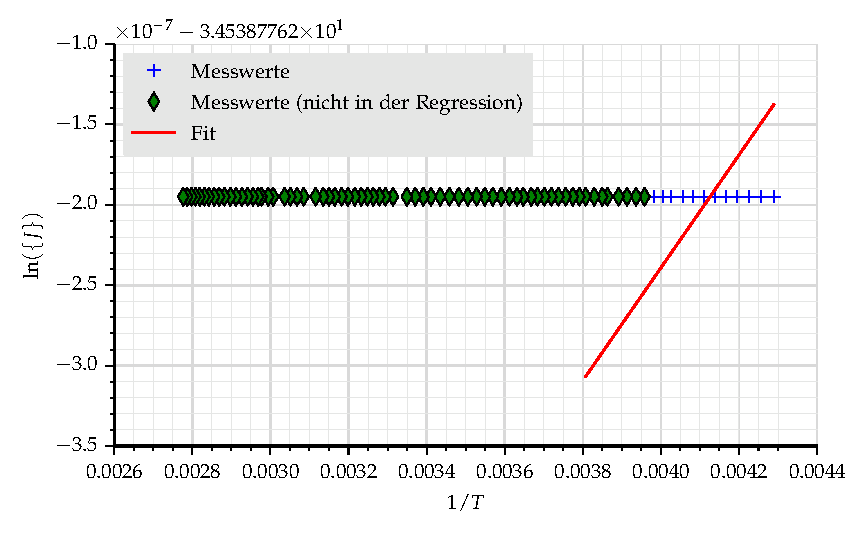
\includegraphics[scale=0.8]{../skript/G1.pdf}
\caption{Darstellung der Messwerte zur Heizrate $b=2.0$ K/min.}
\label{fig:G1}
\end{figure}
\begin{figure}[h]
\centering
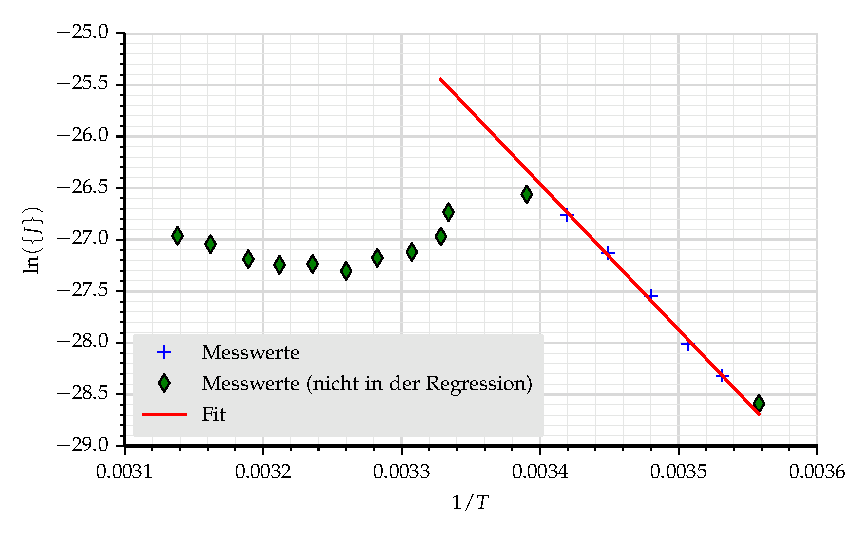
\includegraphics[scale=0.8]{../skript/G2.pdf}
\caption{Darstellung der Messwerte zur Heizrate $b=2.5$ K/min.}
\label{fig:G2}
\end{figure}



Damit ergibt sich
\begin{align}
W_1&= (2.040 \pm 0.020)\times 10^{-20}\text{J}=(0.1273\pm0.0012)\text{ eV}\\
W_2&=  (1.26 \pm 0.14) \times 10^{-20}\text{J}=(0.0786\pm 0.0087)\text{ eV}\quad .
\end{align}
Da bei der Rechnung nur eine fehlerbehaftete Größe (die Steigung der
Ausgleichsgeraden) vorkommt, sind die Fehlerrechnung identisch mit der
zum Mittelwert.
\subsection{Bestimmung von $W$ aus dem gesamten Kurvenverlauf}
Definiere
\begin{equation}
S(T)=\int\limits_T^{T^*} j(T') \text{d}T' \frac{1}{j(T)}
\end{equation}
mit dem letzten gemessenen Wert $T^*$.
Bei konstanter Heizrate gilt
\begin{equation}
\frac{W}{\text{k}_\text{B} T}=\ln S(T)
\end{equation}
mit einer Konstanten $k$. Bei der Berechnung wurde die Näherung
\begin{equation}
S(T)=\int\limits_T^{T^*} j(T') \text{d}T' \approx \sum\limits_{\#\text{Messwerte}} j^n  \hat{b}
\end{equation}
benutzt. Der Index bezieht sich dabei auf den $n$-ten Messwert, $\hat{b}$ ist die
Heizrate in SI-Einheiten. Ein linearer Fit für $\ln(S(T))$ gegen $1/T$ ergibt
%\input{GS1}
%\input{GS2}
\begin{align}
G_{S,1}(x)&= (7.62 \pm 0.13 )\times 10^{3} \,x - (19.04 \pm 0.41)  \\
G_{S,2}(x)&= (8.19 \pm 0.18 )\times 10^{3} \,x - (20.36 \pm 0.53)
\end{align}
Die entsprechenden Abbildungen sind \ref{fig:GS1} und \ref{fig:GS2}.
\begin{figure}[h]
\centering
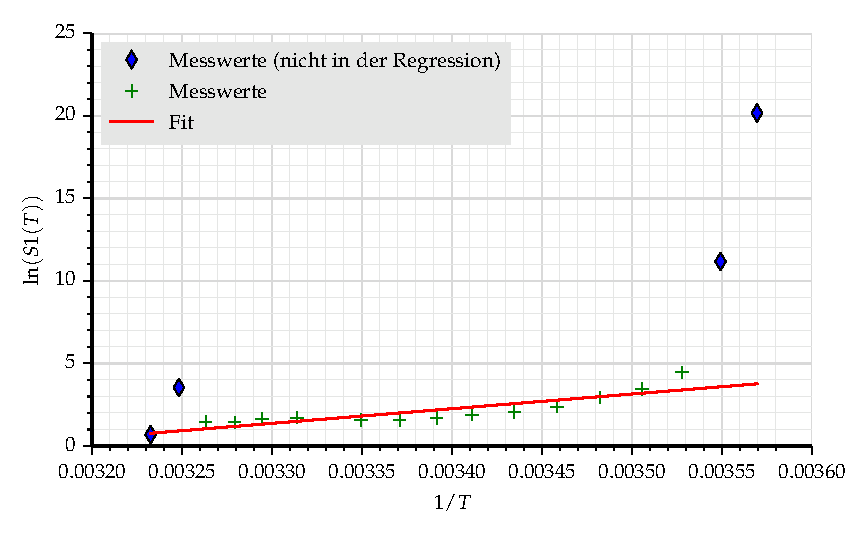
\includegraphics[scale=0.8]{../skript/S1.pdf}
\caption{Darstellung der Messwerte zur Heizrate $b=2.0$ K/min.}
\label{fig:GS1}
\end{figure}
\begin{figure}[h]
\centering
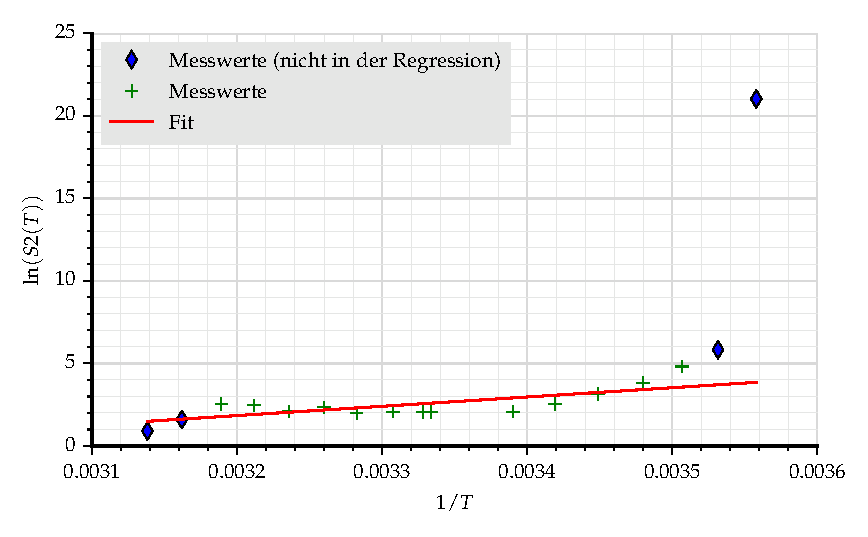
\includegraphics[scale=0.8]{../skript/S2.pdf}
\caption{Darstellung der Messwerte zur Heizrate $b=2.5$ K/min.}
\label{fig:GS2}
\end{figure}
Es folgen
\begin{align}
W_{S,1}&=  (10.51 \pm 0.18)\times 10^{-20}\text{ J} = (0.656\pm 0.011)\text{ eV}\\
W_{S,2}&=  (11.30 \pm 0.25) \times 10^{-20}\text{J} = (0.705\pm 0.016)\text{ eV}\quad .
\end{align}
Da wieder nur eine fehlerbehaftete Größe vorkommt, kann der Fehler wie der
Messwert behandelt werden.

\subsection{Bestimmung der Relaxationszeit $\tau$}
Differentiation von Gleichung \eqref{eq:Stromdichte} ergibt
\begin{equation}
\frac{1}{b}+ \frac{\text{d}}{\text{d}T}\eval_\text{max}\tau(T)=0
\end{equation}
mit $T_\text{max}=\max\{T \}$. Mit
\begin{equation}
 \frac{\text{d}}{\text{d}T}\eval_\text{max}\tau(T) =-\frac{W}{\text{k}_\text{B}
 T^2}
\end{equation}
folgt
\begin{equation}
\tau(T_\text{max})=\frac{\text{k}_\text{B} T_\text{max}^2}{W b} \quad .
\end{equation}
Nun kann mit Hilfe von Gleichung \eqref{eq:relaxationszeit} die Relaxationszeit $\tau_0$
gemäß
\begin{equation}
\tau_0=\tau(T_\text{max})\text{e}^{-\frac{W}{\text{k}_\text{B}T_\text{max}}}
\end{equation}
bestimmt werden.

So ergibt sich
\begin{align}
\tau_{0,1} &=(5.5\pm 2.1)\times 10^{-9} \text{ s} \\
\tau_{0,2} &=(1.50\pm 0.73)\times 10^{-9} \text{ s}
\end{align}

Die Fehlerrechnung geschieht dabei gemäß der Gaußschen Fehlerfortpflanzung.

